%\begin{savequote}[8cm]
%\textlatin{Neque porro quisquam est qui dolorem ipsum quia dolor sit amet, consectetur, adipisci velit...}

%There is no one who loves pain itself, who seeks after it and wants to have it, simply because it is pain...
% \qauthor{--- Cicero's \textit{de Finibus Bonorum et Malorum}}
%\end{savequote}

\chapter{Definitions of key terms} \label{ch:definitions}

\minitoc

\section{Introduction}

Many of the key terms that are ubiquitous in ICF, such as `hotspot' and `ignition', have no single agreed upon definition. This can make it difficult to compare results between different published works, and can mean the use of such terms is ambiguous. This chapter will discuss the definitions for a range of terms and quantities that will be used throughout this thesis, along with the details of exactly how these quantities were evaluated for the simulations presented in later chapters.


\section{Convergence ratio}
The definition of convergence ratio used in this work is 
\begin{equation} \mathrm{CR} =  R_\mathrm{I}/R_\mathrm{HS}, \label{CR} \end{equation} 
where $R_\mathrm{I}$ is the initial interior radius of the DT layer, and $R_\mathrm{HS}$ is the radius of the hotspot. This is the same definition as used in the works by Olson \textit{et al.} \cite{Olson2016} and Zylstra \textit{et al.} \cite{Zylstra2018}, and was selected to ensure compatibility with their findings. This parameter can also be referred to as the `hot-spot convergence ratio', and remains a common definition of convergence ratio for wetted-foam research \cite{Olson2021}.

Other definitions for convergence ratio also exist. Some papers define the initial radius $R_\mathrm{I}$ as the `initial inner radius of the shell' \cite{Craxton2015} or the `initial radius of the DT layer' \cite{Haines2017a}; these are likely the same definition as discussed previously, but the phrasing is potentially ambiguous and could also apply to the DT/ablator interface. Alternatively, a `capsule convergence ratio' is also used where the radius $R_\mathrm{I}$ is instead defined as the outer radius of the capsule, including the CH ablator \cite{Lindl2004}. Further ambiguity is inserted through the $R_\mathrm{HS}$ term. This is often stated as simply the hotspot radius \cite{Olson2016, Olson2021}, but can also be described as the `minimum' hotspot radius, the hotspot radius at peak compression \cite{Craxton2015}, or the stagnated outer radius of the hotspot \cite{Zylstra2018}. These terms are all interpreted to mean the minimum achieved hotspot radius, but it is noted that this does not necessarily occur at the the time of stagnation (itself a poorly defined term) or peak compression. More significant is the ambiguity in how the hostpot radius is identified, as discussed in the following section.

The convergence ratio is often evaluated in simulations where alpha deposition has been turned off \cite{Craxton2015}. This is because alpha deposition leads to increased hotspot pressure, which in turn will decrease the convergence ratio of the capsule. However, if the experimental performance does not match that of the simulations, then this pressure will be reduced and the capsule may converge further before burn begins; and thus using the value derived without alpha deposition represents a worst-case scenario. In this thesis, convergence ratio was calculated with alpha-heating included. This was done for convenience during the capsule optimisation in Chapter \ref{ch-lowCR}, since otherwise two simulations would have been required for each set of parameters (one with alpha-heating to enable calculation of the gain, and one without to enable calculation of the convergence ratio). The focus of this work was largely on achieving break-even, and at these gains the discrepancy between burn and no-burn parameters is minimal (this effect only starts to become significant for gains of around 10 and above \cite{GoncharovPersonalComm}).

\section{Hotspot and shell}

\begin{figure}[ht]
	\centering
	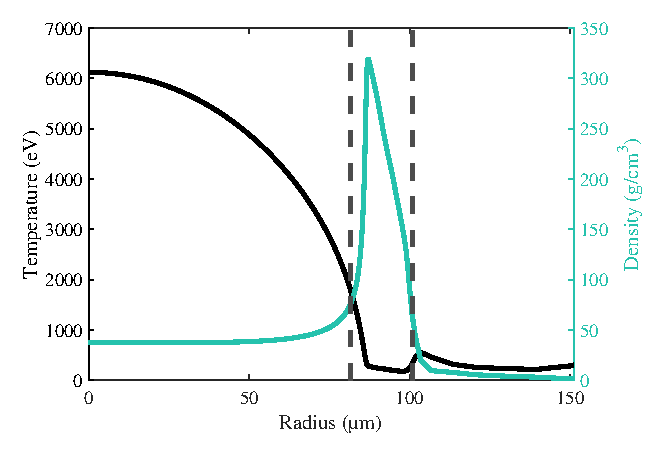
\includegraphics{figures/LowCR/HSDefn.eps}
	\caption{Ion temperature (black) and density (teal) at the time of maximum compression. The two dashed lines indicate the position of the hospot and shell radii using the definitions defined in the text.}
	\label{fig:HsDefn}
\end{figure}

The term `hotspot' is used to refer to the low-density, high temperature region at the centre of the ICF capsule, while the `shell' is the cooler high-density region surrounding it. A plot of a capsule at peak compression, such as that shown in Figure \ref{fig:HsDefn}, clearly shows the relevance of this description. However, where the exact interface between the two lies is not clearly defined. This is particularly true if one wishes to extend the concept of the shell to earlier stages in the implosion before stagnation (for instance, in order to calculate the implosion velocity). There is no accepted definition for this interface, and the definition used in a particular paper is not usually provided; the only definition found was in \cite{Olson2021}, which defined the hotspot as the central region where the temperature was above 5keV. This is not a useful definition for small non-igniting capsules, which despite showing similar temperature and density behaviour to Figure \ref{fig:HsDefn} may not achieve such temperatures anywhere in the capsule. This definition would also poorly describe the capsule in Figure \ref{fig:HsDefn}, where quite a large region of low density material would be considered part of the shell. The definition of these parameters is particularly important, since many other terms (including the convergence ratio) are defined with reference to them.

As such, a new definition for hotspot/shell was identified for this work. The hotspot/shell interface (or `hotspot radius') is defined as the radius at which the density has increased by $1/e^2$ of the difference between the central hotspot density and the peak density in the shell. The shell outer radius is defined as the radius where the density has decreased to $1/e^2$ of the peak value. In Figure \ref{fig:HsDefn} this places the two boundaries at the dashed lines, which matches well with the qualitative description. As this definition is based on density, it works throughout the early stages of the implosion - defining a 'shell' which could be used for the calculation of other quantities. 

\section{Hotspot / shell temperature}
The hotspot and shell temperatures referred to in this thesis are the mass-averaged ion temperatures over the hotspot and shell zones respectively. This (along with the definition for convergence ratio) is a clear example of how defining the hotspot and shell influences other important parameters.

\section{Areal density}

Despite areal density typically being referred to as $\rho R$, which suggests that it is the product of the density and the radius at a given position, the more accepted and commonly used version \cite{Craxton2005, Betti2005, Abu-Shawareb2022} of this quantity is \begin{equation} \rho R = \int_{R_1}^{R_2} \rho \cdot dR, \end{equation} the integral of the density $\rho$ with respect to radius $R$ over the region being considered\footnote{My first paper on this work defined $\rho R$ simply as the mass averaged product of these two quantities, which was replaced with the integral form for subsequent papers.}. Definitions for areal density are often not provided, and some works do indeed discuss $\rho R$ as the product of these two quantities \cite{Atzeni2008}.

In this thesis, $\rho R$ is used to refer to the integral version of this quantity. The major benefit of this definition is that the areal density of different regions sums linearly. This means that the total capsule areal density is the sum of the hotspot areal density and the shell areal density, which makes intuitive sense. Areal density can thus be thought of as a measure of how much DT fuel an alpha particle must move through, when generated at the centre of the capsule and travelling (in a straight line) outwards - which highlights why this quantity is important for alpha absorption, self-heating, and thus gain. It also correlates well to the experimentally determined `neutron averaged' areal density, which is an average of the areal density across the neutron line of travel between the point of generation and the detector.


\section{In-flight aspect ratio}

The definition for the in-flight aspect ratio of the capsule used in this work is \begin{equation} \mathrm{IFAR} = \frac{R_\mathrm{shell}}{t_\mathrm{shell}}, \end{equation}
where $R_\mathrm{shell}$ and $t_\mathrm{shell}$ are the shell radius and thickness. This quantity is evaluated when the capsule has been compressed to two-thirds of it's initial radius, in accordance with the common definition provided in the review article by Craxton \textit{et al.} \cite{Craxton2015} (other works evaluate the IFAR at different times, such as when the shell has converged by a factor of one third \cite{Radha2011}). In the analysis performed in these simulations, the IFAR is evaluated at the point when the shell outer radius (as defined previously) reaches 2/3 of the initial inner radius of the wetted-foam layer. The shell thickness is defined as the shell radius minus the hotspot radius. It should be noted that some works define the shell radius as the position of peak shell density - the definition for $R_\mathrm{shell}$ used in this thesis is larger, and will result in a slightly larger IFAR value than using this alternative definition.

\section{Implosion velocity}

The term `implosion velocity' is typically used to refer to the peak velocity achieved as the capsule implodes. The implosion velocity used in this work was a volume averaged velocity across the material used in the shell. This should more correctly be a mass-averaged implosion velocity, but the difference in these quantities is marginal. 

\section{Laser intensity}

The laser intensity will form an important part in the definition in Chapter \ref{ch-lowCR} for the low-instability regime. However, laser intensity is a function of the area over which the laser acts; if the same power is absorbed over a smaller surface area (i.e. as the capsule radius decreases) the intensity will increase.

In this thesis, the intensity compared to the low-instability criteria is calculated using the initial capsule radius. This was done for convenience; since the initial radius of the capsule is known in advance, the laser power can thus be chosen in order to ensure an appropriate intensity (when using this definition). However, it is also reasonable to assume that the time-dependent intensity at the critical density will not increase much beyond this value, as while the radius decreases the coronal plasma would be expected to decrease the power of the incoming laser through absorption and scattering processes.

\section{Yield, gain and bang time}

Yield (or `fusion yield') throughout this thesis is used to refer to the neutron yield, or the energy carried by the neutrons that will escape the fuel assembly and could thus potentially be captured. \texttt{HYADES} outputs a `total yield' which includes the energy of the alpha particles, and the neutron yield is 80 \% of this value. The number of fusion-generated neutrons can be obtained by dividing the neutron yield by the 14.1 MeV neutron energy \cite{Atzeni2008}.

The term `gain' is used throughout this thesis to refer to the `total' or `target' gain, which is defined as \begin{equation} G = \frac{Y_{tot}}{E_{las}}, \end{equation} where $Y_{tot}$ is the neutron yield and $E_{las}$ is the input laser energy. Alternative variants on gain include capsule gain ($G_{cap} = Y_{tot}E_{abs}$, which compares the yield to only the energy absorbed by the capsule $E_{abs}$) and fuel gain ($G_{fuel} = Y_{tot} / E_{fuel}$, which compares yield instead to the energy absorbed by the DT fuel $E_{fuel}$), both of which are significantly larger \cite{Atzeni2008, Abu-Shawareb2022}.

The bang time of the implosion is defined as the time of maximum neutron generation (i.e. where the peak number of fusion reactions occur) \cite{Craxton2015}.

\section{Adiabat}

The adiabat (or isentrope parameter) of an ICF capsule is used as a measure of the entropy of the cold, highly compressed DT fuel. This is done through comparison with a cold gas with Fermi-degenerate electrons. It is defined as \begin{equation} \alpha = \frac{P(\rho, T)}{P_{deg}(\rho)}, \label{eqn:adiabat} \end{equation} where $P(\rho, T)$ is the pressure of the DT fuel for which the adiabat is calculated, while $P_{deg}(\rho)$ is the pressure for the Fermi-degenerate DT at the equivalent density. This can be calculated using \begin{equation} P_{deg}(\rho) = A_{deg} \rho^{5/3}, \end{equation} where $\rho$ is the density in \unit{\gram\per\centi\meter\cubed}, and $A_{deg} = $ \num{2.17e12} \unit{(\mathrm{erg}/\mathrm{g})/(\mathrm{g}/\mathrm{cm}^3)^{2/3}} for equimolar DT \cite{Atzeni2008}. 

There are multiple ways such a definition can be evaluated, and this is discussed in \cite{Haan2011}. The adiabat is most commonly quoted at the time of peak implosion velocity \cite{Park2014}, but it can also be evaluated post-stagnation. The quoted adiabat value can be either a mass-weighted average, or the minimum adiabat in the DT fuel at that time. If it is an average, the range over which the average is taken can also influence the results. 

An alternative way of calculating adiabat is also provided in \cite{Haan2011}. Here, they instead calculate a mass-averaged entropy at the peak implosion velocity. The equation of state for the DT is then used to calculate the pressure for DT at 1000 \unit{\gram\per\centi\meter\cubed}, on the isentrope defined by that particular entropy value. This calculated pressure is referred to as $P_{cold}$, and replaces the Fermi-degenerate pressure ${P_{deg}(\rho)}$ in the previous equation for adiabat. This is because the cold DT fuel at typical densities achieved in the shell at peak implosion velocity may not be fully ionised, and thus $P_{cold}$ may be lower than ${P_{deg}(\rho)}$. The pressure definition of adiabat does not well account for the density dependence of the DT entropy, and can give behaviour that is non-monotonic in entropy \cite{HainesPersonalComm}. Another alternative definition is to again calculate the mass-averaged entropy of the DT fuel, and then use this value in a fitting formula to calculate the adiabat directly \cite{Haan2011, Haines2022}.

Adiabat does not play a significant role in this thesis, and adiabat values are not reported. In part, this was due to difficulties in this calculation; the adiabat value calculated from Equation \ref{eqn:adiabat} was found to be dependent upon the selection of zones used. \texttt{HYADES} does not return the entropy of the fuel, which means that the alternative definitions could not be used.

%In this work, the reported adiabat is the mass-averaged adiabat of DT in the capsule shell. The minimum adiabat is also calculated, which is the minimum adiabat across the DT zones in the shell. Both of these quantities are calculated as a function of time, and increase as the implosion progresses.

\section{Ignition and break-even}
Of all the ICF parameters, `ignition' is probably the most ambiguous. The National Research Council in 1977 defined ignition as the point at which the fusion energy produced exceeded the laser input; this is easy to understand and describes an important milestone in fusion research, but is not linked to any major physics transition/threshold within the capsule. There are both alternative definitions (for example, it can be defined as the point at which a burn wave starts to propagate through the cold shell \cite{Christopherson2020}), and multiple ways that such definitions can be quantified. When the NIF shot N210808 achieved a yield of 1.3 MJ, this ambiguity meant that it had to be evaluated against nine different criteria in order to claim `ignition' had been achieved \cite{Abu-Shawareb2022}. It was able to satisfy these criteria with high confidence despite not achieving the NIC criteria (which was finally satisfied by the N221214 shot).

Due to this ambiguity and lack of single clear definition, the term `ignition' has been avoided where possible in this thesis. Where it is used, it is done so causally and simply means to achieve a well-performing capsule with high-gain. The term `break-even' is used instead, which has an agreed upon definition of a gain of unity (meaning that it is the same as the NIC ignition criteria, but without the ambiguity).